\documentclass[a4paper, oneside, 11pt]{scrartcl}

% Get the necessary packages for the document.
% Set to english language and utf8.
\usepackage[english]{babel}
\usepackage[utf8]{inputenc}

% Some packages for symbols we need within the tutorial.
\usepackage{dingbat}
\usepackage{marvosym}

% For the sourcecode.
\usepackage{listings}

% Enable Jan's highlighting
% Usage:
% %% preamble
% \usepackage{listings} %% correct name?
\usepackage{lstide}
% \lstset{tabsize=2,captionpos=b,style=default,}
%
%
% %% main
%     \begin{lstlisting}[style=eclipse-java,gobble=6,caption={Simple micro-benchmark in Java}]
%       for (int i = 0; i < 1000; i++) {
%         tin = currentTime();
%         benchmarkedOperation // testtext
%         tout = currentTime();
%       }
%     \end{lstlisting}

% For the links etc.
\usepackage{hyperref} % avh: removed [pdfborder={0 0 0}]

% For the pdf-graphics.
\usepackage{graphicx}

% The steamroller tactics to fix figures and so on.
\usepackage{float}

% This is for tables which are to long to be shown on one page.
\usepackage{longtable}

% This package is for the directory tree structures
\usepackage{dirtree}
\renewcommand*\DTstylecomment{\footnotesize\normalfont\itshape\rmfamily}
\renewcommand*\DTstyle{\footnotesize\sffamily}

% We need this package for some color within the document.
\usepackage{color}

\usepackage[sort,compress,numbers]{natbib} %round,authoryear

% compactitem, compactenum, ...
\usepackage{paralist}


% This is the package for the margin-nodes.
\usepackage[color=white, bordercolor=white]{todonotes}

\usepackage{amsfonts}
\usepackage{setspace}
\usepackage{ae,aecompl}

\usepackage[automark]{scrpage2}

\usepackage[margin=0.5cm,indention=0em,font={small},labelfont={sf,small},format=hang]{caption}

\usepackage[hang,sf]{subfigure}
\subfigcapmargin=1em

%\usepackage{scrhack}

% Get the new commands we defined for this document.
\newcommand{\Kieker}{\textit{Kieker}}
\newcommand{\home}{$\sim$}

% Set the title and everything.
\title{Tutorial for \Kieker:\\ Monitoring and Analysis of Software Behavior}

% Here we go.
\begin{document}
  % We want a table of contents seperated from the rest of the text.
  \maketitle
  \tableofcontents
  \newpage

  \section{Overview}
    \subsection{What is \Kieker?}
      \Kieker\ is a framework\footnote{A framework is sort of a library or code fragment which provides specific and extended functionality.} which allows both programmers and software engineers the monitoring and analysis of program flows and the runtime behavior of java applications. Normal (``plain'') java applications can be arranged with the framework as well as server based java web applications. The framework itself aims to provide an easy managable and maintanable piece of software, which can be included uncomplicated into existing software projects. While \Kieker\ analyzes the own sourcecode reliably, it causes itself only very less overhead during monitoring. \Kieker\ can thereto put whole method calls on a watch, but single statements (e.g. a = a + 1) as well.\\
      Nearly every component of the framework can be extended and adjusted easily to the very own necessities.
      % This is the diagram which shows the single parts of Kieker as one component diagram (the 'satellite').
      \begin{figure}[H]
	\begin{center}
	  \includegraphics[width=1.0\textwidth]{kiekerComponentDiagram.pdf}
	  \caption{The component diagram of \Kieker}
          \label{image:kiekercomponentdiagram}
	\end{center}
      \end{figure}
      As can be seen in figure \ref{image:kiekercomponentdiagram}, the framework consists mainly of two big parts:
      \begin{itemize}
	\item \textbf{\KiekerMonitoring}\\
	  This is the part which is responsible for the logging and the recording of the program behavior. The result of this component are the recorded informations which can then be written into different output streams, like for example into files or into a database.
	\item \textbf{\KiekerAnalysis}\\
	  This part is responsible for the evaluation and visualization of the recorded information. It uses the files (or general any collected data which is available as monitoring records) for the analysis and to produce graphs (e.g. Component-Dependency-Graph).
      \end{itemize}
      Both parts are composed each of three subcomponents which can be used or extended as well with own classes. The rough interaction between the different components is described by the following figure but will be explained furthermore in the course of this tutorial.
      % This is the diagram which shows the interaction between the components and when which component get what kind of input.
      \begin{figure}[H]
	\begin{center}
	  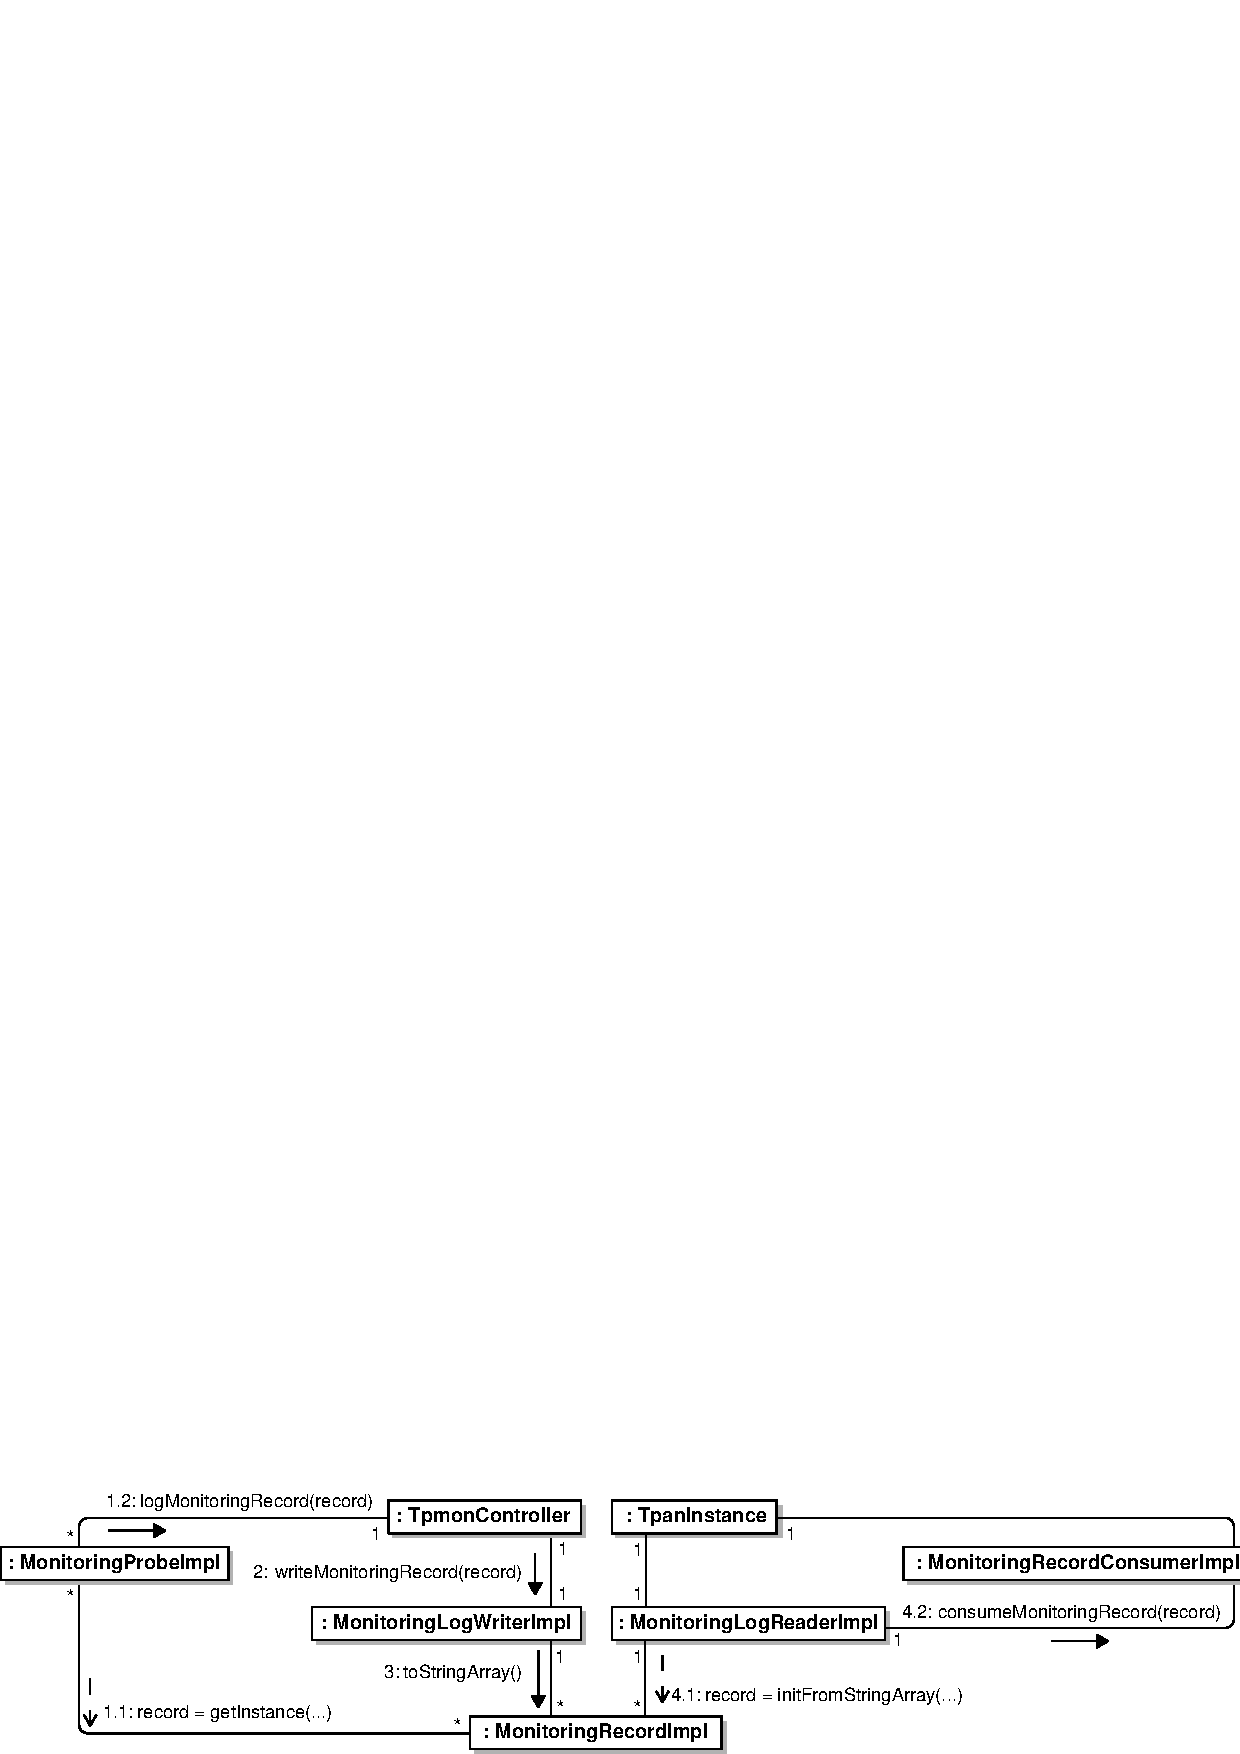
\includegraphics[width=1.0\textwidth]{kiekerCommunications-revisedReArranged-woMonitoringLog-bw.pdf}
	  \caption{Interaction between the components of \Kieker}
	\end{center}
      \end{figure}
      The monitoring probes create either the monitoring records manually or by calling the monitoring controller. The monitoring controller uses the monitoring log writers to persist the given records which can then be later read by a monitoring log reader who creates a monitoring record again. This monitoring records can then be used by the consumer in nearly every way.

    \subsection{What ist the purpose of this tutorial?}
      In this tutorial, we will take a closer look at both, the \textbf{\KiekerMonitoring}- and the \textbf{\KiekerAnalysis}-part. That means, we will describe on the one hand how \KiekerMonitoring\ can be used to mark parts of the own sourcecode for \Kieker\ and to let them execute under surveilance, so that the recorded information can be saved somewhere and on the other hand we will use \KiekerAnalysis\ to process (for example visualize) our recorded data.\\
      We will show how to create and execute a simple example before we go deeper into the single parts of the framework.

  \section{Quickstart}
    \subsection{Downloading and installing \Kieker}
      For the monitoring and analysis of the source code, it is necessary to download the \Kieker\ binaries from \KiekerDownloadUrl\ first. Once that is done, the content of the zip- respectively the tar.gz-file should be extracted to any directory, for example ``$\sim$/kieker'' (under Linux) or ``c:$\backslash$program files$\backslash$kieker'' (under Windows).\\
      That is already enough for the ``installation'' of \Kieker. If desired, the new created path can of course be assigned to an easy remindable environment variable 
      % Note: Maybe it should be described how to do this.

    \subsection{Monitoring}
      Now for the creation of a simple example for the use of the \Kieker\ framework (note: The example is available on the website of \Kieker). It is recommended to create a new working directory (e.g. $\sim$/example) with the following subdirectories:
      \begin{itemize}
	\item src (For the sourcecode files)
	\item lib (For the libraries and needed jar-files)
	\item META-INF (For the configuration files of \Kieker)
	\item build (For the builded class files of Java)
      \end{itemize}
      Before we start with the source code, we need to copy some files from the \Kieker\ directory to our own working directory\footnote{It would be possible to access the required files within the \Kieker\ directory, but the copying will make the compiling much more comfortable.}.
      \begin{itemize}
	\item $\sim$/kieker/dist/\monitoringCtrlJar\ to $\sim$/example/lib/\monitoringCtrlJar
	\item $\sim$/kieker/lib/commons-logging-1.1.1.jar to $\sim$/example/lib/commons-logging-1.1.1.jar
        % Note: Is the log4j.properties really necessary? Seems to work without it.
	\item $\sim$/kieker/META-INF/log4j.properties.example to $\sim$/META-INF/\textbf{log4j.properties}
      \end{itemize}
      The last file is a configuration file, but for a quick start it is already configurated correctly.\\

      We start with creating two directories for our packages:
      % Note: This wouldn't be really necessary, but the package belonging is better visible.
      \begin{itemize}
	\item $\sim$/example/src/mySimpleKiekerExample
	\item $\sim$/example/src/mySimpleKiekerExample/bookstoreTracing
      \end{itemize}
      In the last directory, we create three files: 
      \begin{itemize}
	\item CRM.java
	\item Catalog.java
	\item Bookstore.java
      \end{itemize}
      The file ``Bookstore.java'' should contain of the lines showed in listing \ref{listing:Bookstore.java}.
      % It isn't necessary to do this every time but it makes sure that the listing has the correct format.
      \setJavaCodeListing
      % This will give the code a caption and - more important - a label which we can refer to.
      \lstset{caption=Bookstore.java, label=listing:Bookstore.java}
      % Careful! We load the file directly from the source directory. 
      \lstinputlisting{source-example/manual-monitoring/src/mySimpleKiekerExample/bookstoreTracing/Bookstore.java}
      Listing \ref{listing:Catalog.java} shows the content of ``Catalog.java'' and listing \ref{listing:CRM.java} the content of ``CRM.java''.
      \lstset{caption=Catalog.java, label=listing:Catalog.java}
      \lstinputlisting{source-example/manual-monitoring/src/mySimpleKiekerExample/bookstoreTracing/Catalog.java}
      \lstset{caption=CRM.java, label=listing:CRM.java}
      \lstinputlisting{source-example/manual-monitoring/src/mySimpleKiekerExample/bookstoreTracing/CRM.java}
      The monitoring itself is done manually. Although this is not the strength of \Kieker\ it is pretty good for a quick start.
      % It would be a waste of time to extract the part from the source-file. we do it manually.
      \lstset{caption=Cutting from Bookstore.java, label=listing:cuttingBookstore}
      \begin{lstlisting}
	long tin = TpmonController.getInstance().getTime();
	Bookstore.searchBook();
	long tout = TpmonController.getInstance().getTime();

	KiekerExecutionRecord e = KiekerExecutionRecord.getInstance("mySimpleKiekerExample.bookstoreTracing.Bookstore", "searchBook()", "sessionID", 0, tin, tout, "vnName", 0, 0);
	TpmonController.getInstance().logMonitoringRecord(e);
      \end{lstlisting}
      In this listing can be seen, how the monitoring itself is done. We use the \textit{TpmonController} to get the current time in nano seconds and remember the time before and after a specific method call (in this case: \textit{searchBook()})\footnote{The code between the timekeeping does not need to be a method call of course. It can be ``plain'' code or more than one method call as well.}. These informations are stored in the so called execution record. It gets:
      % I am afraid it's a little bit complicate with the eoi and ess.
      \begin{itemize}
	\item The component (the class) in which the called method is.
	\item The called method.
	\item The session id. In this case we can use any string.
	\item The trace id of the current trace we want to record. Due to the fact, that we follow only one trace, this is zero in all recordings.
	\item The time before the sourcecode which should be measured.
	\item The time after the sourcecode which should be measured.
	\item The name of the current host. This is not very important in this case, because we have only one host. The name can be choosen freely.
	\item The eoi (execution order index). This tells \Kieker\ later the sequence of the different calls. It should be of course unique within a trace.
	\item The ess (execution stack size). This number tells \Kieker\ that the execution was started when the calling stack of the corresponding trace was just the                
              ess.
      \end{itemize}
      For the moment we have to choose the eoi and ess manually. These numbers can be choosen later automaticaly by \Kieker\ of course.\\
      Once the writing is done, we should be able to compile and execute the sourcecode:
      % We need something like the ouput from the bash.
      \setBashListing
      % Note: A little bit long...and the name of the libaries have to be changed manually.
      \begin{lstlisting}
	nils@Laptop:~/example$ javac ./src/mySimpleKiekerExample/bookstoreTracing/Bookstore.java ./src/mySimpleKiekerExample/bookstoreTracing/Catalog.java ./src/mySimpleKiekerExample/bookstoreTracing/CRM.java -classpath ./lib/kieker-monitoring-1.5-trunk_ctrl.jar:./lib/commons-logging-1.1.1.jar -d build/
	nils@Laptop:~/example$ java -Dlog4j.configuration=META-INF/log4j.properties -classpath ./build/:./lib/kieker-monitoring-1.5-trunk_ctrl.jar:./lib/commons-logging-1.1.1.jar mySimpleKiekerExample.bookstoreTracing.Bookstore
      \end{lstlisting}
      If everything worked correctly, there should now be a new directory named ``tpmon-20100605-115948636-UTC'' (just with other numbers) in the default temporary directory (under Linux this should be ``/tmp''). In this directory, there should be a file with the extension ``.dat'' with a content similar to the following:
      % Note: We don't have a suitable listing for 'plain' text. We use the bash listing for the moment.
      \begin{lstlisting}
	$1;1275745883934593403;-1;mySimpleKiekerExample.bookstoreTracing.Catalog.getBook(false);sessionID;0;1275745883931011663;1275745883933424540;vnName;1;1
	$1;1275745883937096236;-1;mySimpleKiekerExample.bookstoreTracing.Catalog.getBook(false);sessionID;0;1275745883935003302;1275745883937075214;vnName;3;2
	$1;1275745883937119354;-1;mySimpleKiekerExample.bookstoreTracing.CRM.getOffers();sessionID;0;1275745883934661568;1275745883937111043;vnName;2;1
	$1;1275745883937128922;-1;mySimpleKiekerExample.bookstoreTracing.Bookstore.searchBook();sessionID;0;1275745883931007961;1275745883937123824;vnName;0;0 
      \end{lstlisting}
      These are the recorded informations from our source code. This data can now be visualized with the help of \Kieker.

    \subsection{Analysis}
      % Here we go...we have to inform the user of the programs he need for the converting. And that means as well, that a window user cannot do this part.
      For the visualization via \Kieker\ we need the both tools graphviz (\url{www.graphviz.org/}) and plotutils (\url{www.gnu.org/software/plotutils/}).\\
      Assume that we already have our recorded informations saved in a ``.dat''-file somewhere for example in the ``tmp``-directory, we can now start with converting these informations into graphs. For the first, we change into our \Kieker\-directory ($\sim$/kieker). It is recommended to create a new directory for the graphs first:
      \begin{lstlisting}
	nils@Laptop:~/kieker$ mkdir /tmp/graphs
      \end{lstlisting}
      The shell-script ''./bin/trace-analysis.sh`` will now do most of the job. It starts the analysis and uses the above-mentioned tools to convert to files into graphs and diagrams.
      \begin{lstlisting}
	nils@Laptop:~/kieker$ ./bin/trace-analysis.sh --plot-Sequence-Diagrams --short-labels -i /tmp/tpmon-20100606-112536844-UTC/ -o /tmp/graphs/
      \end{lstlisting}
	The command ''--plot-Sequence-Diagrams`` tells the shell script to convert our data into a sequence diagram\footnote{Other diagrams and graphs can be plot of course as well. Start trace-analysis.sh without any parameters to see the possible commands.}; with ''--short-labels`` we make sure that the components get a shorter name and the directories after ''-i`` and ''-o`` are the input- and the output-directories. If everything went well, \Kieker\ converted the data into files, which can now converted directly into visual graphs:
	\begin{lstlisting}
	  nils@Laptop:~/kieker$ ./bin/dotPic-fileConverter.sh /tmp/graphs/ svg
	\end{lstlisting}
	The shell script ''./bin/dotPic-fileConverter.sh`` gets the directory with the files and the desired file extension (e.g. svg or png). The resulting graphs should now be available in ''/tmp/graphs`` and should look like figure \ref{image:sequencediagram}
	% This is the simple sequence diagram which results by running the bookstore example; of course without showing the traces etc.
	\begin{figure}[H]
	  \begin{center}
	    \includegraphics[width=0.7\textwidth]{sequenceDiagram.pdf}
            \caption{The resulting sequence diagram}
	    \label{image:sequencediagram}
	  \end{center}
	\end{figure}
	We are now able to monitor source code and to visualize these recorded informations in a simple way.

    \subsection{Using annotations}
      Now we want to monitor whole methods without surrounding the method calls with a block where we keep the time manually. We will now use so called annotations to mark the methods we want to monitor\footnote{To be more precisely: We use annotations which will then be used by the aspect-oriented Java extension named AspectJ to surround the method calls with code blocks which are similar to these, we already used manually.}. As can be seen in the following listing we write the annotation \textit{kieker.monitoring.annotation.TpmonExecutionMonitoringProbe} above the methods to be monitored. 
      \setJavaCodeListing
      \lstset{caption=Bookstore.java, label=listing:Bookstore2.java}
      \lstinputlisting{source-example/annotation-monitoring/src/mySimpleKiekerExample/bookstoreTracing/Bookstore.java}
      Due to the use of AspectJ we need now to copy the file ''META-INF/aop.xml.example`` from our \Kieker\ directory to our working directory to ''META-INF/aop.xml``. This file tells AspectJ which parts of our source code should be monitored. To inform AspectJ about our own annotations, we need another libarary as well. We copy $\sim$/kieker/dist/kieker-tpmon-\version\_ctw.jar to our own example project in $\sim$/example/lib/kieker-tpmon-\version\_ctw.jar\\
      To make sure that every method in our program which is annotated will be monitored, we have to write the following into the ''aop.xml``:
      \setXMLListing 
      \begin{lstlisting}
	<aspectj>
	  <!-- turn verbose on to check which files are instrumented -->
	  <!-- <weaver options="-verbose"/> -->
	  <weaver options="">
	      
	  <!-- The following line is the important one -->
	  <include within="*"/> 

	  <!-- uncomment following to instrument sun jpetstore -->
      \end{lstlisting}
      The compiling is pretty much the same as before (except for some more libraries), but in order to run the program, we have to copy the configuration files into the build-directory.
      % Same as before. If the libraries change, this has to be modified as well.
      \begin{lstlisting}
	nils@Laptop:~/example$ javac ./src/mySimpleKiekerExample/bookstoreTracing/Bookstore.java ./src/mySimpleKiekerExample/bookstoreTracing/Catalog.java ./src/mySimpleKiekerExample/bookstoreTracing/CRM.java -classpath ./lib/kieker-monitoring-1.5-trunk_ctrl.jar:./lib/commons-logging-1.1.1.jar -d build/
	nils@Laptop:~/example$ cp -r ./META-INF/ ./build/META-INF
	nils@Laptop:~/example$ java -Dlog4j.configuration=META-INF/log4j.properties -javaagent:lib/aspectjweaver-1.6.6.jar -Dorg.aspectj.weaver.showWeaveInfo=true -Daj.weaving.verbose=true -classpath ./build/:./lib/kieker-monitoring-1.5-trunk_ctrl.jar:./lib/commons-logging-1.1.1.jar:./lib/kieker-monitoring-1.5-trunk_ctw.jar mySimpleKiekerExample.bookstoreTracing.Bookstore
      \end{lstlisting}


  \section{\KiekerMonitoring}
    \subsection{Configuration}
      The monitoring part of \Kieker\ can be configured using the configuration file named ''\monitoringPropertiesFile``. This file should be copied for use to the directory ''META-INF`` of the own project and should - like the ''aop.xml`` - be copied during compiling. In order to inform \Kieker\ about this file, the following parameter should be used for the JVM:
      \begin{lstlisting}
	-Dkieker.monitoring.properties=META-INF/kieker.monitoring.properties
      \end{lstlisting}
      Most of the variables are self-explanatory and some of them will be explained in the following.

    \subsection{Records}
      % They are not really only part of the monitoring components, but they have to be mentioned somehow.
      As we already saw, the records are the objects which store the monitored informations somehow. They are not really part of \KiekerMonitoring\ but in order to the use in the following, we will examine them.\\
      If we want to implement an own record, it should be extend the already existing class \textit{kieker.common.record.AbstractMonitoringRecord}. The record should be able to put his complete content into an array (of Object] so that the other components of \Kieker\ are able to persist and load the data and should of course provide a method to restore the content from an array. The following listing shows a simple record implementation which has fields for the class and the method that is called.
      \setJavaCodeListing
      \lstset{caption=MyRecord.java}
      \lstinputlisting{source-example/monitoring-and-analysis-with-own-components/src/mySimpleKiekerExample/bookstoreTracing/MyRecord.java}

    \subsection{Probes}
      The probes are responsible for the decision which (and where) informations should be recorded. Technically we already implemented them by surrounding the method calls with the correct statements to clock, to produce the records and to deliver these records to the monitoring controller. Other specific controller could for example record only the amount of delivered bytes between methods or record only every second method call as well.\\
      We already used the annotations to make the monitoring much more comfortable and could also implement own annotations for AspectJ, but this won't be explained in this tutorial, because it would simply go beyond the scope.

    \subsection{Writers}
      \hypertarget{monitoringlogwriters} 
      The so called \textit{monitoring log writers} (they can be seen as well in figure \ref{image:kiekercomponentdiagram}) are the parts of \Kieker\ which are responsible for writing and serializing the recorded informations into files, databases and so on. In other words: They get an instance of \textit{AbstractKiekerMonitoringRecord} and produce an output of any nature whatsoever.\\
      Of course there are already some writers implemented, as can be seen in figure \ref{image:writers}.
      % This is the diagram with the different types of writers.
      \begin{figure}[H]
	\begin{center}
	  \includegraphics[width=0.5\textwidth]{kieker_writerimpls.pdf}
	  \caption{The inheritance hierarchy of the current implemented monitoring log writers}
	  \label{image:writers}
	\end{center}
      \end{figure}
      As the quick start part already showed it, every monitored record is sent to the \textit{TpmonController} which itself calls the current writer. The writer uses for example the \textit{toArray()} method of the record to get the informations stored by the record as handable array. The writer is then able to write these objects for example into a file.\\
      The implementation of an own writer class is quiet simple and can be done by implementing the interface \textit{kieker.monitoring.writer.IMonitoringLogWriter}. The following listing shows an example writer which uses a named pipe\footnote{The class \textit{MyNamedPipeManager} will be shown in the appendix of this tutorial.} to write the given records directly into the memory.
      \setJavaCodeListing
      \lstset{caption=MyWriter.java}
      \lstinputlisting{source-example/monitoring-and-analysis-with-own-components/src/mySimpleKiekerExample/bookstoreTracing/MyWriter.java}
      It is necessary to tell \KiekerMonitoring\ which writer should be used. This can be done in the already mentioned file ''\monitoringPropertiesFile``:
      \setBashListing
      \begin{lstlisting}
	monitoringDataWriter=mySimpleKiekerExample.bookstoreTracing.MyWriter
	monitoringDataWriterInitString=somePipe

	# 1.1.5 [property has been removed:] Use monitoring record type IDs

	# 1.1.6 Queue Size used to store Monitoring Records
	# Asyncronous Writers need to store Monitoring Records in an internal Queue.
	# This parameter defines the Number of Records cached. If this number is exceeded
	# Kieker will terminate with a Queue Full Exception!
	#
	asyncRecordQueueSize=8000
      \end{lstlisting}
      The first property decides which writer should be used. If we don't use any of the already implemented writers, we have to deliver the whole name of the class of the writer. The second property is an init string which can be used to initialize the writer in any way. In this case we use this parameter to tell the writer which pipe should be used. The third property is just important for asyncronous writers. It must be pointed out that the resulting init string our writer gets is of the form ''somePipe $|$ asyncRecordQueueSize=8000``. 


    \section{\KiekerAnalysis}
      % The analysis works a little bit different, that is why we explain it here.
      \KiekerAnalysis\ is the part of \Kieker\ which is responsible for the analysis, consisting of the reader, the consumer and the analysis instance itself. After we stored somewhere our records, we need to read them again somehow. This is task of the reader. Whatever we want to do with these informations is task of the consumers. They can for example evaluate, process or visualize the data. The analysis instance concerns about the lifetime and registration of the other parts.\\
      The analysis consists roughly of the following steps:
      \begin{enumerate}
	\item Create one (or more) analysis instance.
	\item Set the reader of this instance and line it with the necessary informations to read the stored records.
	\item Register the consumers who should do something with the recorded data.
	\item Start the analysis instance.
      \end{enumerate}
      % For the moment we don't have ANY configuration for the analysis part. This has to be done in the program.
      % \subsection{Configuration}

      \subsection{Readers}
	The \textit{monitoring log readers} (their position can be found in figure \ref{image:kiekercomponentdiagram}) are the direct counterpart to the \hyperlink{monitoringlogwriters}{\textit{monitoring log writers}}. While the writers get a record and write them in files or somewhere else, the readers take the writen data (from files, databases and so on) and convert them into a suitable instance of \textit{AbstractKiekerMonitoringRecord}. That means, that whenever we are implementing a new writer, we should also implement a corresponding reader. If we want for example save our recorded informations in a database, we have to be capable of reading these stored informations from the database again.\\
	Again there are some readers already implemented in \Kieker\ but we can implement an own reader as well. The following diagram shows the rough hierarchy.
	% This is the diagram with a simple reader hierarchy.
	\begin{figure}[H]
	  \begin{center}
	    \includegraphics[width=0.5\textwidth]{kieker_readerimpls.pdf}
	    \caption{The simple inheritance hierarchy of some currently implemented monitoring log readers}
	    \label{image:readers}
	  \end{center}
	\end{figure}
	The implementing of an own reader is nearly the same as the implementing of the writer, but to keep things simple, it is recommended to extend the already implemented AbstractKiekerMonitoringLogReader, because otherwise it would be necessary to implement the used observer pattern of the reader. By using the methods of the abstract class \textit{kieker.analysis.reader.AbstractMonitoringLogReader}, the task of delivering a new record to the consumers can be delegated to the super class.\\
	The following listing shows a simple reader which reads a stored record from the pipe. If there is nothing on the pipe to be read, the reader waits 4 seconds at maximum before it terminates.
	\setJavaCodeListing
	\lstset{caption=MyReader.java}
	\lstinputlisting{source-example/monitoring-and-analysis-with-own-components/src/mySimpleKiekerExample/bookstoreTracing/MyReader.java}

      \subsection{Consumers}
	The consumers are the parts of \Kieker\ which work with the records that have been loaded by the reader. There can be (theoretically) an infinite number of consumers which produce any kind of output. A consumer can be programmed by implementing the interface \textit{kieker.analysis.plugin.IMonitoringRecordConsumerPlugin} and implementing the necessary methods. Our following example consumer takes the given record and writes the content to the default output stream.
	\setJavaCodeListing
	\lstset{caption=MyConsumer.java}
	\lstinputlisting{source-example/monitoring-and-analysis-with-own-components/src/mySimpleKiekerExample/bookstoreTracing/MyConsumer.java}

      \subsection{The analysis}
	To put everything together, the following listing shows how to use the above-mentioned components.
	% It is not necessary to show the whole method.
	\setJavaCodeListing
	\begin{lstlisting}
	  AnalysisInstance ai = new AnalysisInstance();
	  MyReader reader = new MyReader();
	  reader.init("somePipe");
	  ai.setLogReader(reader);
	  ai.registerPlugin(new MyConsumer());
	  ai.run();
	\end{lstlisting}

  \section{Appendix}
    \subsection{Used classes}
      \subsubsection{MyNamedPipeManager and MyPipe}
	\setJavaCodeListing
	\lstset{caption=MyNamedPipeManager.java}
	\lstinputlisting{source-example/monitoring-and-analysis-with-own-components/src/mySimpleKiekerExample/bookstoreTracing/MyNamedPipeManager.java}

	\setJavaCodeListing
	\lstset{caption=MyPipe.java}
	\lstinputlisting{source-example/monitoring-and-analysis-with-own-components/src/mySimpleKiekerExample/bookstoreTracing/MyPipe.java}

    \subsection{Example logs}
    \subsection{Shortcut via ant}
    \subsection{Libraries}
      The following tables shows all libraries which are used by \Kieker\ and explains them in short words.
      \begin{center}
\begin{longtable}{|p{0.4\textwidth}|p{0.5\textwidth}|}
\hline 
Filename & Description\\
\hline
\hline 
aspectjrt-1.6.11.jar & This jar-file contains the runtime library for AspectJ programs.\\
\hline 
aspectjtools-1.6.11.jar & This package contains the tools (the AspectJ Compiler and Browser) for AspectJ.\\
\hline 
aspectjweaver-1.6.11.jar & This jar contains the weaver-agent for the aspect-oriented-extension for Java named AspectJ.\\
\hline 
commons-cli-1.2.jar & Apache Commons CLI provides a simple API for working with the command line arguments and options.\\
\hline 
commons-logging-1.1.1.jar & Apache Commons Logging is a thin adapter allowing configurable bridging to other, well known logging systems.\\
\hline 
cxf-api-2.2.10.jar & Apache CXF is an open source services framework.  \\
\hline 
cxf-common-utilities-2.2.10.jar & This package contains different classes for Apache CXF.\\
\hline 
cxf-rt-bindings-soap-2.2.10.jar & This package contains necessary files to use Apache CXF as well with the Simple Object Access Protocol (SOAP).\\
\hline 
cxf-rt-core-2.2.10.jar & This library contains the Apache CXF Runtime Core. \\
\hline 
derby.jar & Apache Derby is a lightweight database written in Java which can also be used as an embedded database. This library contains the necessary drivers for the database as well as the database management system itself.\\
\hline 
jms-1.1.jar & Java Message Service is an API to send and receive messages within a client and to control so called Message Oriented Middleware (MOM).\\
\hline 
jndi-1.2.1.jar & The Java Naming and Directory Interface is an API which provides methods for multiple naming and directory services. It can be used for example to register disposed files in a network and to allow other part of a Java program to use them for RMI calls.\\
\hline 
junit-4.5.jar & This jar-file contains the necessary classes for the JUnit-tests, which can be used to test automatically Java classes.\\
\hline 
log4j-1.2.15.jar & Apache log4j is a framework for the logging of messages, errors and exceptions in Java applications.\\
\hline 
servlet-api.jar & The Java Servlet API supplies protocols to let applications respond for example to HTTP requests.\\
\hline 
sigar-1.6.3.jar & Hyperic SIGAR (System Information Gatherer) provides a Java API to system inventory and monitoring data (Memory, CPU etc.). In addition to the Jar file, it is required to add corresponding platform-specific native libraries to the classpath, which can be downloaded from~\cite{HypericSigarWebsite}. Kieker's \dir{lib/} folder already includes such libraries for Linux/Windows for the x86~architecture (\file{libsigar-x86-linux.so} and \file{sigar-x86-winnt.[dll|lib]}.\\
\hline 
spring.jar & The spring framework delivers different methods and classes to make the handling with Java/Java EE easier.\\
\hline 
spring-web.jar & This library contains the web application context, multipart resolver, Struts support, JSF support and web utilities for the spring framework.\\
\hline 
\end{longtable}
\label{tabular:libraries}
\end{center}

    \subsection{Troubleshooting}

\end{document}
 
